\documentclass[11pt,a4paper]{article}

% ---------------------------------------------------------------------------
% Laboratório 404 — artigo científico/tecnológico
% Autor: William da Silva Vianna (Instituto Federal Fluminense)
% Compilação: pdflatex -> bibtex -> pdflatex -> pdflatex  (ver build.sh)
% ---------------------------------------------------------------------------

\usepackage[utf8]{inputenc}
\usepackage[T1]{fontenc}
\usepackage[brazil]{babel}
\shorthandoff{"}

% Área de texto ampliada (a classe article em A4 tem \textwidth de apenas
% 360pt, insuficiente para as tabelas e diagramas do artigo).
\usepackage[margin=2.5cm]{geometry}

\usepackage{graphicx}
\graphicspath{{figures/}}
\usepackage{booktabs}
\usepackage{array}
\usepackage{float}
\usepackage{amsmath}
\usepackage{amssymb}
\usepackage{tikz}
\usetikzlibrary{arrows.meta,positioning,shapes.geometric,fit}
\usepackage{pgfplots}
\pgfplotsset{compat=1.18}
\usepackage[round]{natbib}
\usepackage[hidelinks]{hyperref}

% Metadados do PDF: o título interno casa com o nome do arquivo de
% distribuição (artigo-laboratorio-404.pdf); o título acadêmico completo
% permanece em pdfsubject e no cabeçalho do artigo.
\hypersetup{
  pdftitle={Artigo - Laboratório 404},
  pdfauthor={William da Silva Vianna},
  pdfsubject={Artigo científico/tecnológico; Laboratório 404: um jogo 3D educacional com uma IA local restrita ao mundo: arquitetura, processo incremental e validação automatizada},
  pdfkeywords={jogos sérios; grandes modelos de linguagem; inferência local; Godot; Blender; desenvolvimento orientado a especificação}
}

\title{Laborat\'orio 404: um jogo 3D educacional com uma IA local\\
restrita ao mundo --- arquitetura, processo incremental e valida\c{c}\~ao automatizada}

\author{William da Silva Vianna\\Instituto Federal Fluminense}

\date{Setembro de 2026}

% [A CONFIRMAR] e-mail de contato, campus/cidade e ORCID do autor.

\emergencystretch=2em

\begin{document}

\maketitle

\begin{abstract}
\noindent
Jogos educacionais podem se beneficiar de grandes modelos de linguagem (LLMs)
capazes de dialogar com o jogador, mas integrar esses modelos a um jogo real
imp\~oe desafios de seguran\c{c}a (a IA n\~ao deve controlar o jogo), de
desempenho (infer\^encia local em hardware modesto) e de engenharia (manter o
processo rastre\'avel em um desenvolvimento de autor \'unico assistido por
agentes de IA). Este artigo relata o projeto, a implementa\c{c}\~ao e a
valida\c{c}\~ao do \textbf{Laborat\'orio 404}, um jogo 3D
educacional/ficcional no qual a IA \textbf{ARIA} administra uma instala\c{c}\~ao
subterr\^anea e conversa com o jogador sem nunca controlar o estado do mundo.
O prot\'otipo foi constru\'ido em seis provas de conceito incrementais
(POC~1 a POC~6) sobre Godot~4.5, Blender~5.2.1, um adaptador Python (FastAPI)
e o Ollama com modelo local; as respostas da IA s\~ao restritas a cinco
inten\c{c}\~oes validadas em duas camadas, com \textit{fallback} textual. A
valida\c{c}\~ao combinou especifica\c{c}\~ao rastre\'avel, su\'ite automatizada
\textit{headless} e evid\^encias visuais. Resultados: 211 verifica\c{c}\~oes
Godot e 16 testes Python aprovados; cena 3D com 342 n\'os e 37 materiais
(1.018,7~KB em GLB) executando a 60~FPS (limitado por \textit{vsync}) em GPU
integrada AMD Radeon Graphics a 1280$\times$720; respostas de ARIA com o modelo
local \texttt{llama3.1:8b} entre 12,9~s e 22~s em tr\^es medi\c{c}\~oes. As
limita\c{c}\~oes incluem aus\^encia de estudo com usu\'arios, valida\c{c}\~ao
manual de hardware pendente e n\~ao execu\c{c}\~ao do modelo-alvo
\texttt{llama3.2:3b}. Os artefatos (c\'odigo, especifica\c{c}\~ao, capturas e
v\'ideo de demonstra\c{c}\~ao) s\~ao p\'ublicos.
\end{abstract}

\noindent\textbf{Palavras-chave:} jogos s\'erios; jogos educacionais; grandes
modelos de linguagem; infer\^encia local; Godot; desenvolvimento orientado a
especifica\c{c}\~ao.

\section{Introdução}
\label{sec:introducao}

Jogos sérios são jogos cujo propósito principal não é o puro entretenimento
\citep{abt1970serious} e que, nas últimas duas décadas, consolidaram-se como
instrumentos de educação, treinamento e simulação \citep{zyda2005from,
laamarti2014overview}. A literatura sobre aprendizagem sustenta que bons jogos
incorporam princípios pedagógicos --- identidade, experimentação ativa,
problemas bem ordenados e retroalimentação imediata --- que podem ser
aproveitados também na educação formal \citep{gee2003what}. Construir um jogo
com esse propósito, porém, exige mais do que uma boa ideia: exige arquitetura,
processo e evidências de que o artefato realmente funciona.

Nos últimos anos, grandes modelos de linguagem (LLMs) passaram a ocupar papel
de destaque em jogos, seja gerando conteúdo, seja animando personagens ou
apoiando o próprio desenvolvimento \citep{gallotta2024largelanguage}. Os
resultados são promissores, mas trazem dois problemas práticos. O primeiro é de
\emph{controle}: agentes que decidem e executam ações podem alterar o estado do
jogo de formas imprevisíveis --- em \emph{Generative Agents}, os personagens
planejam, refletem e agem com grande autonomia \citep{park2023generative} e, em
\emph{Voyager}, o agente escreve e executa código para progredir
\citep{wang2023voyager}; ambos dependem de modelos de grande porte remotos ou
de infraestrutura substancial. O segundo é de \emph{reprodutibilidade}: é raro
que um projeto de jogo com IA descreva, com o mesmo cuidado, o processo de
desenvolvimento, os critérios de aceitação e as evidências de teste.

Este artigo enfrenta esses dois problemas em um caso real: o \textbf{Laboratório
404}, um jogo 3D educacional/ficcional no qual uma IA local, \textbf{ARIA},
administra uma instalação subterrânea e conversa com o jogador --- mas nunca
controla o jogo. O protótipo foi desenvolvido em seis provas de conceito
incrementais (POC~1 a POC~6) sobre Godot~4.5 (gameplay), Blender~5.2.1 (assets
3D), um adaptador Python/FastAPI e o Ollama com modelo local. A IA recebe
contexto do jogo e devolve apenas texto e uma intenção restrita a cinco valores
validados em duas camadas independentes; qualquer desvio vira \texttt{NONE} e
o jogo usa uma resposta de \emph{fallback}. O desenvolvimento foi documentado
como especificação executável (requisitos funcionais e não funcionais, critérios
de aceitação no formato DADO/QUANDO/ENTÃO e matriz de rastreabilidade) e
validado por uma suíte automatizada \emph{headless}.

O trabalho parte de três perguntas de pesquisa:

\begin{itemize}
  \item \textbf{RQ1 (arquitetura):} como integrar uma LLM local a um jogo 3D de
  modo que ela enriqueça o mundo e a narrativa sem, em nenhum momento,
  controlar o estado do jogo?
  \item \textbf{RQ2 (viabilidade):} é possível manter jogabilidade a 60~FPS e
  conversa local com latência tolerável em um computador sem GPU dedicada?
  \item \textbf{RQ3 (processo):} como conduzir e documentar esse
  desenvolvimento --- de autor único, assistido por agentes de IA --- de forma
  rastreável e reprodutível?
\end{itemize}

As contribuições são: (i) um padrão de arquitetura de \emph{IA diegética com
capacidade limitada}, com dupla validação de intenções e \emph{fallback}
(\autoref{sec:metodologia}); (ii) um processo incremental orientado a
especificação, com evidências automatizadas e visuais; (iii) uma implementação
completa e aberta --- código, especificação, capturas e vídeo de demonstração
--- disponível publicamente \citep{lab404repo,lab404video}; e (iv) resultados
empíricos de execução em GPU integrada, incluindo as latências medidas da
conversa com o modelo local.

O restante do artigo está organizado assim: a
\autoref{sec:fundamentacao} revisa os trabalhos relacionados; a
\autoref{sec:metodologia} descreve o processo, a arquitetura, o pipeline de
assets, a integração da IA e a estratégia de validação; a
\autoref{sec:resultados} apresenta os resultados; a \autoref{sec:discussao}
discute interpretação, comparação, limitações e implicações; e a
\autoref{sec:conclusao} conclui.

\section{Fundamentação teórica e trabalhos relacionados}
\label{sec:fundamentacao}

\subsection{Jogos sérios e educacionais}

O termo \emph{jogos sérios} popularizou-se a partir da definição de Abt:
jogos com um propósito educacional explícito, que não são feitos apenas para
divertir --- embora possam ser divertidos \citep{abt1970serious}. A pesquisa em
aprendizagem com jogos mostrou que bons jogos já incorporam, de forma orgânica,
princípios que a escola persegue: identidade, experimentação, risco controlado,
regras claras e retroalimentação constante \citep{gee2003what}. A visão de
simulação virtual como base para jogos, e dos jogos como ferramenta de
treinamento, foi consolidada na transição de simulação para realidade
virtual \citep{zyda2005from}. Revisões mais recentes organizam o campo por
aplicação (saúde, defesa, educação, planejamento) e apontam que a avaliação de
impacto segue sendo um desafio metodológico
\citep{laamarti2014overview}. [REFERÊNCIA NECESSÁRIA: diretrizes
contemporâneas de avaliação de jogos sérios em contextos escolares.]

\subsection{Grandes modelos de linguagem em jogos}

O levantamento de Gallotta \emph{et al.} mapeia os papéis que LLMs podem
assumir em jogos --- geração de conteúdo, personagens, apoio ao projeto,
testes --- e discute limites práticos, como custo, latência e confiabilidade
\citep{gallotta2024largelanguage}. Duas limitações recorrentes interessam
diretamente a este trabalho: (a) modelos grandes exigem infraestrutura
relevante ou serviços externos; e (b) quanto maior a autonomia concedida ao
modelo, maior a superfície de risco sobre o estado do jogo.

\subsection{Agentes generativos e autonomia}

\emph{Generative Agents} propôs agentes que armazenam experiências em linguagem
natural, sintetizam reflexões e planejam comportamento, produzindo
comportamento social emergente e verossímil em um ambiente interativo
\citep{park2023generative}. \emph{Voyager} levou a autonomia adiante em
Minecraft: um currículo automático, uma biblioteca de habilidades em código e
um mecanismo iterativo de prompting com retroalimentação do ambiente; o agente
aprende continuamente sem ajuste de parâmetros, consultando um modelo externo
\citep{wang2023voyager}. Esses trabalhos demonstram o potencial da autonomia,
mas também a distância entre esse desenho e um jogo educacional em que cada
ação precisa ser previsível, auditável e barata de executar. Neste artigo, a
escolha é deliberadamente oposta: a IA conversa, comenta e sugere; quem age é
sempre o motor do jogo.

\subsection{Inferência local}

Executar o modelo na própria máquina elimina dependência de serviços externos,
dispensa chaves de API e mantém o conteúdo no computador do usuário; o Ollama
é uma ferramenta consolidada para esse cenário \citep{ollama2026}. O custo é a
latência: modelos menores rodam em hardware modesto, mas geram respostas em
escala de segundos, o que restringe seu uso a interações conversacionais (por
turnos) em vez de reações em tempo real. [REFERÊNCIA NECESSÁRIA: estudo
comparativo de latência de LLMs locais em hardware sem GPU dedicada.]

\subsection{Processo de desenvolvimento}

Práticas como desenvolvimento orientado a testes e a especificações propõem
que critérios verificáveis sejam escritos antes da implementação.
[REFERÊNCIA NECESSÁRIA: fontes canônicas sobre desenvolvimento orientado a
especificação.] No contexto deste projeto, essas práticas foram adaptadas a um
fluxo de trabalho assistido por agentes de IA: a especificação, os requisitos e
os critérios de aceitação são os artefatos que restringem cada iteração de
implementação, e a suíte automatizada é o juiz comum entre autor humano e
agente. O uso de servidores MCP (\emph{Model Context Protocol}) para dar ao
agente acesso controlado a ferramentas --- no caso, a cena do Blender --- é
parte desse fluxo \citep{lab404repo}.

\subsection{Síntese e lacuna}

A literatura concentra-se, de um lado, em agentes autônomos e capazes de agir
\citep{park2023generative,wang2023voyager} e, de outro, em visões amplas sobre
o papel das LLMs em jogos \citep{gallotta2024largelanguage}. O que este
trabalho investiga é a combinação menos explorada: \emph{uma IA diegética, com
capacidade formalmente limitada, executada localmente e integrada a um jogo
educacional completo, com processo de desenvolvimento documentado e
evidências de validação}. É nessa lacuna que se posicionam as contribuições
descritas na \autoref{sec:metodologia}.

\section{Materiais e métodos}
\label{sec:metodologia}

\subsection{Estratégia de desenvolvimento}

O projeto seguiu um processo orientado a especificação, adaptado ao contexto de
autor único assistido por agentes de IA. Antes do código, foram fixados: uma
constituição com princípios não negociáveis; um roadmap de seis provas de
conceito; uma especificação com requisitos funcionais (FR) e não funcionais
(NFR), critérios de aceitação no formato DADO\slash QUANDO\slash ENTÃO e uma matriz de
rastreabilidade requisito--teste; e regras permanentes de interação para
agentes de IA \citep{lab404repo}.

Duas regras estruturaram o trabalho. A primeira é a \emph{Regra de Ouro}: cada
POC termina em uma versão executável e demonstrável, com caminho de teste
reproduzível --- o protótipo nunca fica quebrado entre etapas. A segunda é a
proibição de índices de botão no gameplay (FR-001/NFR-005): o jogo consome
apenas ações semânticas de um \emph{Input Map} (\texttt{move\_forward},
\texttt{interact}, \texttt{pause} e outras), o que manteve o mesmo código
funcional para teclado e para o adaptador USB de PlayStation 1, cuja
enumeração de eixos e botões varia conforme o hardware.

Os agentes de IA trabalharam dentro dessas restrições: a especificação e os
critérios de aceitação funcionavam como contrato de cada iteração e a suíte
automatizada, como juiz comum. Um servidor MCP (\emph{Model Context Protocol})
no editor dava ao agente acesso controlado à cena do Blender para modelagem
assistida \citep{lab404repo}.

\subsection{Ambiente e ferramentas}

A \autoref{tab:ambiente} resume o ambiente de desenvolvimento e execução,
verificado por comando na máquina de referência. As versões reportadas são
exatamente as que produziram os resultados da \autoref{sec:resultados}; o
projeto mantém um passo de importação de recursos (GLB e áudio) executado por
linha de comando, necessário na primeira execução de cada clone.

\begin{table}[H]
\centering
\caption{Ambiente de desenvolvimento e execução (verificado em 2026-09-10).}
\label{tab:ambiente}
\begin{tabular}{@{}>{\raggedright\arraybackslash}p{38mm}>{\raggedright\arraybackslash}p{104mm}@{}}
\toprule
Item & Versão / configuração \\
\midrule
Sistema operacional & Ubuntu 24.04.4 LTS \\
CPU / GPU & AMD Ryzen 7 5700U com Radeon Graphics (GPU integrada) \\
Memória & 30 GiB \\
Motor de jogo & Godot 4.5 (\texttt{4.5.stable.official.876b29033}), renderer \texttt{gl\_compatibility} \\
Modelagem 3D & Blender 5.2.1 LTS \\
Linguagem do adapter & Python 3.12.3 \\
Bibliotecas do adapter & FastAPI 0.141.1; Uvicorn 0.52.4; Pydantic 2.13.5; requests 2.34.2 \\
Inferência local & Ollama; modelo-alvo \texttt{llama3.2:3b}; validação com \texttt{llama3.1:8b} \\
Formato de assets & glTF 2.0 binário (GLB) \\
\bottomrule
\end{tabular}
\end{table}

O motor de jogo~\citep{godot2026} concentra gameplay, física, interface, áudio e
persistência; o Blender~\citep{blender2026} produz os assets exportados em
GLB~\citep{khronos2026gltf}; o adaptador usa
FastAPI~\citep{fastapi2026}, Pydantic~\citep{pydantic2026} e
Uvicorn~\citep{uvicorn2026}; e a inferência local é feita pelo
Ollama~\citep{ollama2026}. Os efeitos sonoros são gerados por um script do
próprio projeto, sem conteúdo de terceiros.

\subsection{Arquitetura do sistema}

A \autoref{fig:arquitetura} apresenta a arquitetura. O jogo é um processo
Godot que consome assets exportados do Blender e consome \emph{input} de
teclado e joystick por ações semânticas. A conversa com a IA nunca é feita
diretamente pelo motor: passa por um processo separado (o adaptador), acessível
por HTTP em \texttt{localhost}, que valida a entrada, monta o prompt com a
personalidade versionada e o estado do jogo, chama o Ollama e valida a saída.
Separar a IA do jogo em processos distintos tem duas consequências práticas:
o jogo continua jogável com a IA desligada (respostas de \emph{fallback}) e a
falha de qualquer elo não derruba a aplicação.

\begin{figure}[H]
\centering
\begin{tikzpicture}[
  font=\small,
  box/.style={draw, rounded corners=2pt, align=center, inner sep=5pt,
              minimum height=10mm, fill=black!4},
  arr/.style={-{Stealth[length=2.2mm]}, semithick},
  lbl/.style={font=\scriptsize, inner sep=1.5pt}
]
\node[box] (blender) {Blender 5.2.1};
\node[box, right=12mm of blender] (glb) {GLB/glTF};
\node[box, right=12mm of glb, minimum width=40mm] (godot) {\textbf{Godot 4.5}\\ \scriptsize gameplay, física, UI, áudio, save};
\node[box, above=11mm of godot, minimum width=40mm] (inputs) {\scriptsize Teclado e joystick USB PS1};
\node[box, below=15mm of godot, minimum width=40mm] (adapter) {\textbf{Adaptador FastAPI}\\ \scriptsize validação, intenções, fallback};
\node[box, right=16mm of adapter, minimum width=24mm] (ollama) {\textbf{Ollama}\\ \scriptsize LLM local};

\draw[arr] (blender) -- (glb);
\draw[arr] (glb) -- (godot);
\draw[arr] (inputs) -- node[lbl, right]{\scriptsize Input Map} (godot);
\draw[arr] ([xshift=-2.5mm]godot.south) -- node[lbl, left]{\scriptsize pergunta + estado} ([xshift=-2.5mm]adapter.north);
\draw[arr] ([xshift=2.5mm]adapter.north) -- ([xshift=2.5mm]godot.south);
\draw[arr] (adapter) -- node[lbl, above]{\scriptsize prompt} (ollama);
\draw[arr] ([yshift=-2.5mm]ollama.west) -- ([yshift=-2.5mm]adapter.east);
\node[lbl, below=1mm of adapter, text width=42mm, align=center]
  {\scriptsize resposta: texto + intenção restrita};
\end{tikzpicture}
\caption{Arquitetura do Laboratório 404. A IA vive fora do processo do jogo: o adaptador é a fronteira onde entrada e saída são validadas.}
\label{fig:arquitetura}
\end{figure}

\subsection{Pipeline de assets (Blender para GLB)}

A cena 3D foi modelada no Blender sob convenções fixas: 1 unidade do Blender
equivale a 1 metro (NFR-002); objetos usam prefixos por função
(\texttt{ENV\_} para ambiente, \texttt{PROP\_} para equipamentos,
\texttt{DEC\_} para decoração, \texttt{NPC\_} para personagens); e a colisão é
embutida no próprio asset por meio do sufixo \texttt{-col}, que o importador
do Godot converte em corpo estático, mantendo a malha visível original para
renderização. As transformações são aplicadas antes da exportação, e o GLB
resultante é importado pela linha de comando do motor, sem edição manual de
cena. O detalhamento progressivo da sala --- luminárias, letreiros,
sinalização, mobiliário e um NPC completo --- foi conduzido nessas convenções e
medido ao final (\autoref{sec:resultados}).

\subsection{ARIA: IA local com intenções restritas}

O núcleo do desenho de segurança está na \autoref{fig:conversa}. A IA devolve
sempre um objeto estruturado com texto, intenção e confiança; a intenção é
sanitizada no adaptador e novamente no cliente do jogo. O conjunto permitido é
deliberadamente pequeno:

\begin{verbatim}
ALLOWED_INTENTS = {"HINT", "DIAGNOSE", "LORE",
                   "STATUS", "NONE"}
\end{verbatim}

Qualquer valor fora desse conjunto --- inclusive ruído devolvido pelo modelo
--- é convertido para \texttt{NONE} (FR-017, CA-010). A resposta também é
limitada em forma e conteúdo: mensagem de entrada entre 1 e 2000 caracteres
(erro 422 quando inválida), \emph{timeout} de 30~s na chamada ao Ollama e
resposta de \emph{fallback} textual em caso de exceção (FR-018, NFR-004). O
cliente no jogo espera um pouco mais que o adaptador e, se nada chegar,
também usa texto pré-definido --- ou seja, a IA pode estar lenta ou ausente sem
comprometer a jogabilidade (CA-009). A personalidade de ARIA (identidade,
regras, tons de voz e texto de \emph{fallback}) fica em um arquivo JSON
versionado, não espalhada em código (FR-020), e o estado do jogo é injetado no
prompt como contexto factual. Em nenhum ponto a IA recebe permissão de escrever
estado, abrir portas ou alterar física (FR-021, NFR-006).

\begin{figure}[H]
\centering
\begin{tikzpicture}[
  font=\small,
  node distance=6mm,
  etapa/.style={draw, rounded corners=2pt, align=center, inner sep=4pt,
               fill=black!4, text width=92mm},
  guarda/.style={etapa, fill=black!12, draw=black, thick},
  arr/.style={-{Stealth[length=2mm]}, semithick}
]
\node[etapa] (a) {Terminal de ARIA: o jogador digita a mensagem};
\node[etapa, below=of a] (b) {Cliente HTTP no jogo (GDScript): espera limitada e resposta de fallback pré-definida};
\node[etapa, below=of b] (c) {Adaptador FastAPI: valida a entrada (Pydantic, 1 a 2000 caracteres), monta o prompt com personalidade versionada e estado do jogo};
\node[etapa, below=of c] (d) {Ollama (local): gera JSON com texto, intenção e confiança (timeout de 30 s)};
\node[guarda, below=of d] (e) {Sanitização em duas camadas: intenção fora do conjunto permitido vira NONE; o jogo nunca executa comandos da IA};
\draw[arr] (a) -- (b);
\draw[arr] (b) -- (c);
\draw[arr] (c) -- (d);
\draw[arr] (d) -- (e);
\end{tikzpicture}
\caption{Cadeia de uma mensagem até a resposta. Cada elo falha de forma segura: o pior caso é um texto de fallback, nunca um travamento ou uma ação não prevista.}
\label{fig:conversa}
\end{figure}

\subsection{Conteúdo e jogabilidade}

O arco do vertical slice começa com a chegada do técnico à instalação e um
tutorial de controles dentro do jogo; segue pela missão
\texttt{RESTAURAR\_COMUNICACAO} (\autoref{fig:missao}); passa por um corredor
que dá acesso a uma ala procedural gerada a partir de uma semente
determinística (mesma semente, mesmo laboratório; conectividade garantida por
construção) e culmina no núcleo de ARIA, com um epílogo de três escolhas. Ao
longo do percurso, o mundo reage ao jogador: luzes mudam conforme o estado da
energia, uma câmera de segurança passa a acompanhar o jogador depois que a
energia volta, um NPC comenta o estado dos equipamentos e a ARIA muda de tom
quando um alerta é ignorado. O progresso é serializável em arquivo local
(save/load) e a ambiência sonora é contínua, com efeitos para interações,
porta, alarme e erro.

\begin{figure}[H]
\centering
\begin{tikzpicture}[
  font=\scriptsize,
  node distance=4mm,
  s/.style={draw, rounded corners=2pt, align=center, inner sep=3pt,
            fill=black!4, text width=20mm},
  arr/.style={-{Stealth[length=1.8mm]}, semithick}
]
\node[s] (a) {buscar fusível F-17};
\node[s, right=of a] (b) {buscar módulo RS-404};
\node[s, right=of b] (c) {instalar no painel};
\node[s, right=of c] (d) {reiniciar CLP};
\node[s, right=of d] (e) {diagnosticar bomba};
\node[s, right=of e] (f) {abrir a porta B1};
\foreach \x/\y in {a/b, b/c, c/d, d/e, e/f} {
  \draw[arr] (\x) -- (\y);
}
\end{tikzpicture}
\caption{A missão principal em seis passos dependentes e ordenados. Cada passo só é aceito quando o anterior está concluído.}
\label{fig:missao}
\end{figure}

\subsection{Validação automatizada e evidências}

A validação combina três instrumentos. O primeiro é a suíte de testes
\emph{headless}: cada POC tem uma cena de teste que instancia o jogo, executa
interações reais (mover, coletar, instalar, conversar, salvar) e verifica o
estado resultante, sem depender de janela ou de intervenção manual. O segundo
é um conjunto de testes de API em Python que exercita o adaptador com
requisições válidas e inválidas, inclusive limites e \emph{fallback}. O
terceiro é um arnês de captura de tela: uma cena que posiciona o jogador em
poses pré-determinadas, opcionalmente conclui a missão e salva imagens
automáticas em 1280$\times$720 --- usado para produzir as evidências visuais
deste artigo.

Itens que exigem presença física ou julgamento humano são explicitamente
separados: operação de mouse com captura de cursor, calibração do adaptador
PS1 em hardware real e o playthrough humano de ponta a ponta (CA-013). Esses
itens estão declarados como pendentes nos artefatos do projeto, e não são
tratados como concluídos por inferência.

\section{Resultados}
\label{sec:resultados}

\subsection{Artefatos entregues}

Ao final do ciclo, as seis provas de conceito estavam implementadas e
demonstráveis de forma independente, conforme a Regra de Ouro: fundação
jogável; laboratório funcional com missão completa; ARIA integrada por adapter;
mundo reativo; laboratório procedural; e o vertical slice com tutorial,
persistência, áudio e epílogo. O material público inclui o código-fonte, a
especificação com requisitos e critérios de aceitação, as capturas de tela
usadas neste artigo e um vídeo de demonstração de 1~min~08~s
(1280$\times$768 a 30~fps) que percorre a missão do POC~2
\citep{lab404repo,lab404video}. O conjunto de scripts do jogo soma cerca de
2.400 linhas de GDScript (contagem bruta de linhas, incluindo comentários) e a
suíte de testes do motor, cerca de 1.300 linhas.

\subsection{Suíte automatizada}

A \autoref{tab:verificacoes} detalha as verificações por POC. No total, 210 a
211 verificações do motor mais 16 testes do adapter, todas aprovadas na
execução de referência. A variação de uma verificação no POC~3 é esperada: com
o adapter no ar, um dos casos de \emph{fallback} dá lugar à validação da
resposta real do modelo.

\begin{table}[H]
\centering
\caption{Verificações automatizadas por prova de conceito (suíte \emph{headless}, execução de referência de 2026-09-10).}
\label{tab:verificacoes}
\begin{tabular}{@{}l >{\raggedright\arraybackslash}p{96mm} r@{}}
\toprule
POC & Escopo validado & Verificações \\
\midrule
1 & Fundação jogável: input semântico, movimento, câmera, pausa, HUD, diagnóstico de input & 77 \\
2 & Laboratório funcional: interação, inventário, porta, missão, sala modelada & 34 \\
3 & ARIA: adapter, terminal, timeout, validação de intenção, fallback & 25--26 \\
4 & Mundo inteligente: NPC, luzes por energia, tom da ARIA, memória em camadas & 21 \\
5 & Laboratório procedural: determinismo por semente, conectividade entre módulos & 23 \\
6 & Vertical slice: tutorial, missão completa, save/load, áudio, epílogo & 30 \\
Adapter & API de ARIA (Python): contratos, validação, erros e limites & 16 \\
\midrule
Total & & 210--211 + 16 \\
\bottomrule
\end{tabular}
\end{table}

\begin{figure}[H]
\centering
\begin{tikzpicture}
\begin{axis}[
  ybar,
  width=0.92\textwidth,
  height=5.4cm,
  bar width=9pt,
  ymin=0,
  ylabel={verificações},
  symbolic x coords={POC1,POC2,POC3,POC4,POC5,POC6,Adapter},
  xtick=data,
  nodes near coords,
  every node near coord/.append style={font=\scriptsize},
  tick label style={font=\small},
  label style={font=\small},
]
\addplot[fill=black!35] coordinates {
  (POC1,77) (POC2,34) (POC3,26) (POC4,21) (POC5,23) (POC6,30) (Adapter,16)
};
\end{axis}
\end{tikzpicture}
\caption{Distribuição das verificações automatizadas por etapa do projeto.}
\label{fig:verificacoes}
\end{figure}

\subsection{Cena 3D e desempenho}

A sala do laboratório foi exportada em um único arquivo GLB com 342 nós, 37
materiais e 35 objetos de colisão embutidos, totalizando 1.018,7~KB; o emissivo
dos materiais usa a extensão \texttt{KHR\_materials\_emissive\_strength}, o que
permitiu acender telas e sinalizações sem estourar o branco no renderizador
compatível. A \autoref{fig:sala} mostra o resultado em jogo. O desempenho
medido foi de 60~FPS limitados por \emph{vsync} a 1280$\times$720 na GPU
integrada, inclusive após o detalhamento da cena (342 objetos e 34 elementos
de iluminação/letreiros), mantendo o critério NFR-001. Métricas de tempo de
quadro por percentil não foram coletadas
[MEDIÇÃO DE FRAME TIME NÃO REALIZADA].

\begin{figure}[H]
\centering
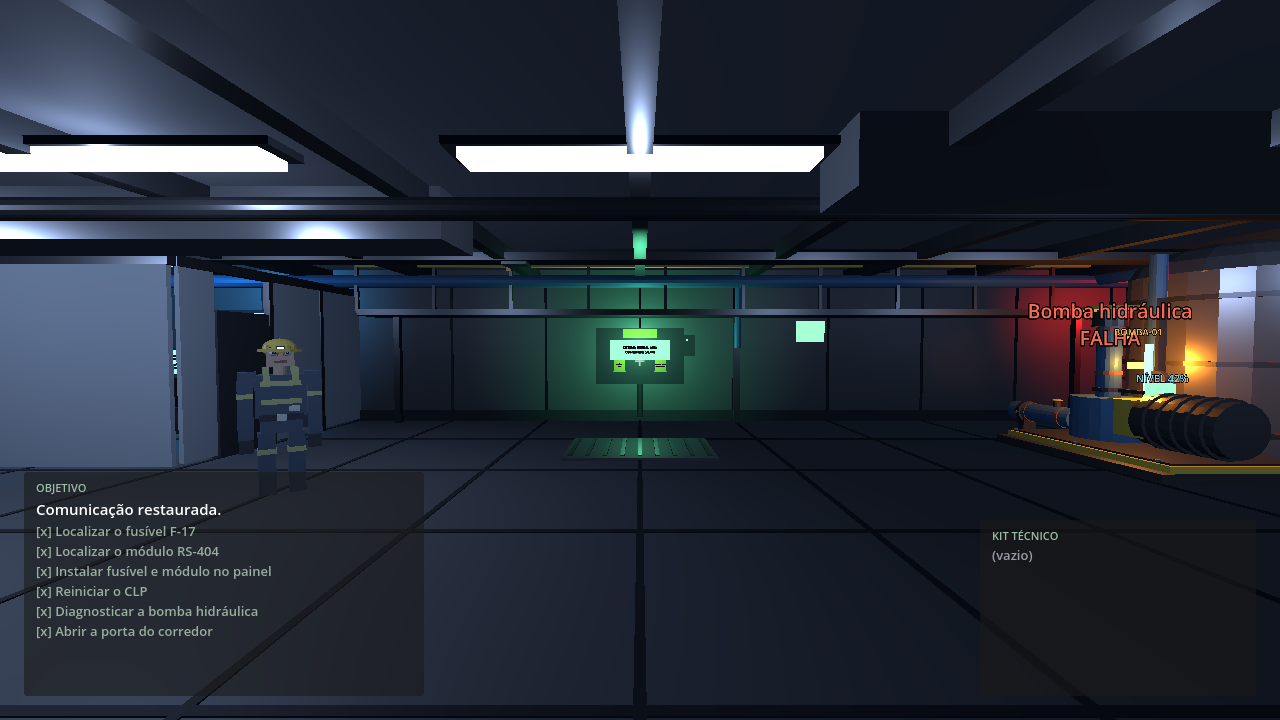
\includegraphics[width=0.92\textwidth]{sala-energizada.png}
\caption{Vista da sala do Laboratório 404 com a energia restaurada: luminárias do teto acesas, câmera de segurança ativa, porta B1 liberada e letreiros das estações. Captura do jogo em 1280$\times$720 (fonte: material do projeto).}
\label{fig:sala}
\end{figure}

\subsection{Conversa com ARIA}

O critério de aceitação central --- receber uma resposta útil ou um
\emph{fallback} em tempo limitado, sem travar o jogo --- foi validado em três
contextos com o modelo local \texttt{llama3.1:8b}
(\autoref{tab:latencia}). As latências ficaram entre 12,9~s e 22,0~s; a
partida fria é o pior caso, e o teste no jogo (\autoref{fig:terminal}) passou
5 de 5 verificações de integração. O modelo-alvo declarado na especificação,
\texttt{llama3.2:3b}, não estava instalado no ambiente de referência, de modo
que os números representam o desempenho com um modelo maior e mais lento ---
ou seja, são um limite superior conservador para o alvo. Com o adapter ou o
modelo fora do ar, o jogo responde com texto de \emph{fallback} e intenção
\texttt{NONE}, conforme projetado (CA-009).

\begin{table}[H]
\centering
\caption{Latências medidas da conversa com ARIA usando modelo local \texttt{llama3.1:8b}.}
\label{tab:latencia}
\begin{tabular}{@{}>{\raggedright\arraybackslash}p{64mm} l r >{\raggedright\arraybackslash}p{36mm}@{}}
\toprule
Contexto & Intenção & Latência & Observação \\
\midrule
Chamada direta ao adapter (partida fria) & DIAGNOSE & 22,0 s & confiança 0,9 \\
Terminal de ARIA no jogo & STATUS & 16,1 s & captura em \texttt{docs/images} \\
Cliente no jogo (teste ao vivo) & HINT & 12,9 s & 5 de 5 verificações \\
\bottomrule
\end{tabular}
\end{table}

\begin{figure}[H]
\centering
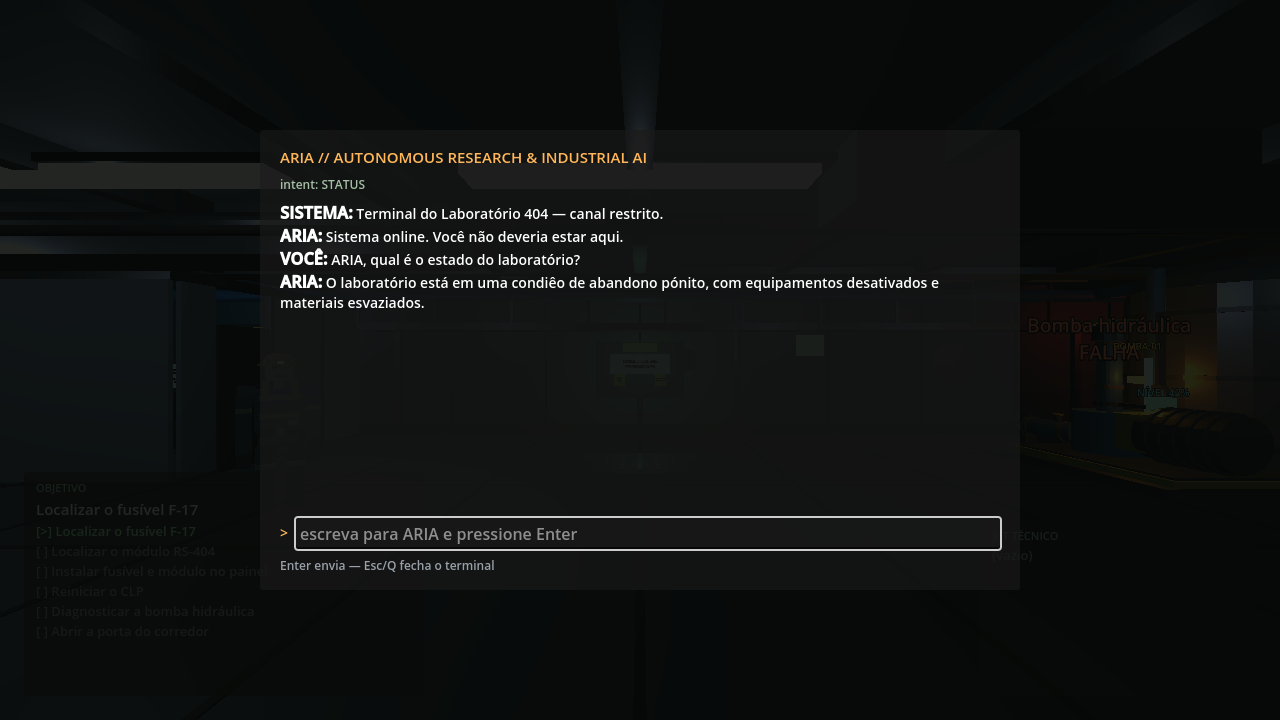
\includegraphics[width=0.92\textwidth]{aria-terminal.png}
\caption{Terminal de ARIA no jogo: a pergunta do jogador e a resposta do modelo local (latência de 16,1~s, intenção \texttt{STATUS}). Fonte: material do projeto.}
\label{fig:terminal}
\end{figure}

\section{Discussão}
\label{sec:discussao}

\subsection{Interpretação dos resultados}

Os resultados respondem afirmativamente às três perguntas de pesquisa, dentro
do escopo de um protótipo. Sobre a arquitetura (RQ1): a combinação de processo
separado, contrato estruturado e sanitização em duas camadas mostrou-se
suficiente para que a IA participasse do mundo --- dando dicas, diagnosticando
equipamentos, comentando o estado do laboratório e mudando de tom --- sem
receber qualquer capacidade de alterar o estado do jogo. O pior caso
observado, em todas as falhas induzidas nos testes, foi uma resposta de
\emph{fallback}: nunca um travamento, nunca uma ação não prevista.

Sobre a viabilidade (RQ2): a jogabilidade manteve-se em 60~FPS limitados por
\emph{vsync} na GPU integrada, com a cena detalhada (342 objetos, 37
materiais), e a conversa local apresentou latência de 12,9~s a 22,0~s com um
modelo de 8 bilhões de parâmetros. Essa ordem de grandeza é adequada a uma
interação conversacional por turnos --- o terminal de ARIA --- e inadequada a
reações em tempo real, o que reforça a decisão de projeto de não colocar a IA
no laço de controle. Sobre o processo (RQ3): a especificação com critérios
verificáveis e a suíte automatizada permitiram que cada etapa fosse aceita ou
rejeitada com base em evidência, e não em impressão; as seis etapas fecharam
com a suíte verde.

\subsection{Comparação com a literatura}

O contraste com os trabalhos de referência é deliberado. \emph{Generative
Agents} e \emph{Voyager} investigam o que acontece quando se concede ao modelo
autonomia de decisão e de execução \citep{park2023generative,wang2023voyager};
o Laboratório 404 investiga o oposto --- quanto valor narrativo e pedagógico se
obtém mantendo a IA estritamente consultiva. Essa escolha dialoga com o
levantamento de Gallotta \emph{et al.}, que destaca custo, latência e
confiabilidade como limites práticos das LLMs em jogos
\citep{gallotta2024largelanguage}: aqui esses limites não foram eliminados,
foram convertidos em restrições de projeto (intenções finitas, \emph{fallback}
obrigatório, inferência local). Não há, neste trabalho, comparação quantitativa
com os sistemas citados, pois os alvos são diferentes (agência aberta versus
assistência limitada) [ESTUDO COMPARATIVO NÃO REALIZADO].

\subsection{Limitações e ameaças à validade}

\begin{itemize}
  \item \textbf{Estudo de caso único, sem usuários:} o trabalho é uma
  descrição de projeto e uma validação técnica; não mede aprendizagem nem
  experiência do jogador. O playthrough humano de ponta a ponta (CA-013)
  permanece pendente [ESTUDO DE USUÁRIO NÃO REALIZADO].
  \item \textbf{Amostra pequena de latência:} as três medições da
  \autoref{tab:latencia} são informativas, não experimentais; não há repetição
  controlada, variação de carga ou comparação entre modelos. O modelo-alvo
  \texttt{llama3.2:3b} não foi executado.
  \item \textbf{Ambiente:} os números de desempenho valem para a máquina da
  \autoref{tab:ambiente}; a validação em joystick PS1 físico e o uso de mouse
  capturado seguem manuais. Durante o desenvolvimento, dois atritos de ambiente
  exigiram documentação dedicada: o confinamento do pacote do motor bloqueava o
  acesso a dispositivos de entrada até a conexão explícita da permissão de
  joystick, e o servidor de áudio mantinha um estado de mudo por aplicativo que
  silenciava apenas o jogo. Ambos os casos foram diagnosticados e estão
  registrados como solução de problemas no material do projeto
  \citep{lab404repo} --- são exemplos de ameaças à reprodutibilidade que
  costumam passar em branco em relatos de jogos.
  \item \textbf{Empacotamento:} a geração de um executável independente
  (FR-033) estava bloqueada pela ausência dos modelos de exportação do motor no
  ambiente; o critério permanece aberto.
\end{itemize}

\subsection{Implicações}

Para quem projeta jogos educacionais, o caso sugere que a IA generativa pode
entrar em cena como personagem consultivo --- e não como agente --- com
latência de segundos e execução local, sem abrir mão de previsibilidade. Para
quem pesquisa agentes em jogos, o desenho oferece um ponto de comparação: os
mesmos modelos que rendem mais quando recebem autonomia também rendem valor
narrativo quando recebem limites explícitos. Por fim, para a prática de
desenvolvimento, o experimento sugere que um projeto de autor único assistido
por agentes de IA pode manter rastreabilidade quando a especificação e os
testes precedem a implementação --- e quando cada promessa do resumo é
verificável por um comando.

\section{Conclusão}
\label{sec:conclusao}

Este artigo descreveu o projeto, a implementação e a validação do Laboratório
404, um jogo 3D educacional/ficcional no qual uma IA local participa do mundo
sem controlá-lo. O objetivo foi atingido no nível de protótipo: as seis provas
de conceito foram concluídas e demonstráveis, a suíte automatizada cobre 210 a
211 verificações do motor e 16 testes do adapter, todas aprovadas, e o jogo
roda a 60~FPS (limitados por \emph{vsync}) em GPU integrada, mantendo conversa
local com latência entre 12,9~s e 22,0~s.

As contribuições práticas são o padrão de \emph{IA diegética com capacidade
limitada} --- processo separado, contrato estruturado e sanitização em duas
camadas ---, o processo incremental orientado a especificação com evidências
automatizadas e visuais, e os artefatos públicos que permitem reproduzir e
auditar cada afirmação quantitativa deste texto \citep{lab404repo,lab404video}.

As limitações são conhecidas e declaradas: ausência de estudo com usuários,
medições de latência em pequena amostra, validação manual de hardware
pendente, empacotamento independente ainda não gerado e modelo-alvo menor não
executado. Como trabalhos futuros, pretende-se: (i) executar e comparar o
\texttt{llama3.2:3b} com o modelo usado aqui; (ii) concluir o empacotamento e a
demonstração sem intervenção do desenvolvedor (FR-033); (iii) realizar o
playthrough humano de ponta a ponta e, depois, um estudo controlado com
usuários em contexto educacional; e (iv) ampliar o conteúdo do vertical slice
mantendo a mesma disciplina de evidências.


\section*{Agradecimentos}
O autor agradece a si mesmo --- pela teimosia de levar este projeto at\'e o fim.

\bibliographystyle{plainnat}
\bibliography{references}

\end{document}
